\documentclass[12pt]{extarticle}
\usepackage[francais]{babel}
\usepackage[utf8]{inputenc}
\usepackage{graphicx}
\usepackage{color}
\usepackage{hhline}
\usepackage{multirow}
\usepackage{fancyhdr}
\usepackage{lastpage}
\usepackage{enumitem}

\addto\captionsfrench{\def\tablename{{\textsc{Tableau}}}}

\author{Emmanuel Mollard \\ Antoine Tardy \\ Léa Cruciani \\ Marion Bouvier}
\title{Cahier des charges\\Mytho-Logic}
\date{\today}

\pagestyle{fancy}
\renewcommand\headrulewidth{1pt}
\renewcommand{\footrulewidth}{1pt}
\cfoot{\thepage/\pageref{LastPage}}

\begin{document}

\begin{center}\large
	Cahier des charges \vspace{0.5cm}
\end{center}

\begin{center}\Huge\bfseries
	\underline{Mytho-Logic} \vspace{1cm}
\end{center}

\begin{center}\footnotesize
	Emmanuel Mollard, Antoine Tardy \\ Léa Cruciani, Marion Bouvier, Thibault Trembleau
\end{center}

\begin{figure}[!h]
	\center
	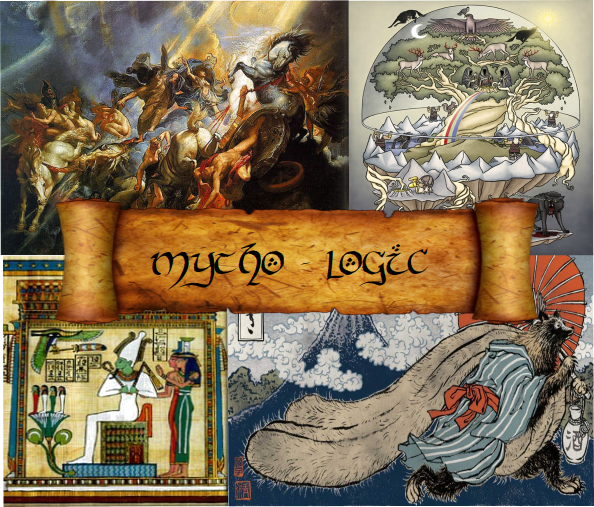
\includegraphics[width=0.8\textwidth]{logo1}
\end{figure}

\newpage

\tableofcontents

\newpage

\section{Introduction}\large

En tant qu’étudiants d’Epita une tâche nous incombe. Une tâche de la plus grande importance qui décidera de notre destin. En effet nous avons 4 mois pour créer un jeu ! Malgré les périples qui nous attendent tout au long de cette aventure notre petite équipe composée de 5 valeureux guerriers est prête et motivée à relever ce défi pour vous immerger dans un nouveau monde ! Heureusement pour eux le grand mage noir Unity détenteur du langage C\# leur viendra en aide. Ce recours à la magie vous transformera en demi-Dieu et vous mènera dans des terres inconnues regorgeant de créatures mythologiques. Et quoi de mieux quand vous arrivez dans des terres inconnues peuplées de créatures plus étranges les unes que les autres que de livrer des combats ? Eh bien… le clan MYONYTOR composé de ces 5 fameux guerriers vous invite à prendre part à la bataille et à affronter d’autres joueurs à l’aide de votre propre armée de créatures. Mais attention demi-Dieu l’environnement auquel vous ferez face est semé d’embûches ! Il faudra user de logique, de ruse, et de stratégie pour venir à bout de vos adversaires sur le champ de bataille.

\vspace{0.5cm}
\begin{center}\bfseries
	À vous de jouer demi-Dieu !
\end{center}

\newpage

\section{Présentation du projet}

\subsection{Contexte}

Pour notre projet de S2 nous avons choisis de créer un jeu vidéo car nous voulions savoir comment un jeu vidéo est créé ?On y joue souvent et on trouvait intéressant de connaître l’envers du décors : le code, l’organisation du travail, la répartition des tâches et le travail d’équipe qui encadrent un jeu vidéo. De plus cela doit être satisfaisant de voir que des personnes jouent et apprécient notre projet. Vouloir créer un jeu, c’est bien beau, mais.. quel type de jeu ? Arcade, stratégie, guerre, RPG ? Il y a-t-il une histoire ? Si oui, quelle est-elle ? Un ou plusieurs joueurs ?

Nous avons donc cherché différentes idées qui pourraient nous amener à la création de notre jeu et de son concept.

\subsection{Les sources d'inspiration}

Nous avons décidé de nous inspirer de différents jeux que nous affectionnons comme Heartstone, Dofus, ou encore Civilization. A chacun de ces jeux nous avons pris un élément du gameplay qui nous susciter de l’intérêt :

\begin{itemize}[label=\textbullet]
	\item Heathstone : \newline Le système du mana que le joueur utilise pour invoquer une carte nous servira à limiter les attaques de nos personnages.
	\item Civilization : \newline Ce qui nous a le plus intéresser c’est la carte du jeu hexagonale car on trouvait que c’était une manière esthétique d’inclure des cases dans un plateau de jeu et cela donnerait plus de possibilités de déplacement et d’attaque à nos personnages.
	\item Dofus : \newline Nous avons sélectionner Dofus pour son point de vue sur le jeu. Une vue de trois quart pour que le joueur puisse prendre en compte tous les éléments présents sur le plateau du jeu. Le système de combat se fait lui aussi sur une map avec des cases mais elles étaient carrées. Alors que nous elles seront hexagonales.
	\item Diplomacy : \newline Cette fois-ci c’est le gameplay qui nous a le plus attiré. En effet dans ce jeu l’actualisation du mouvement des personnages ce fait en simultané et non un à un. On trouvait cela donc très intéressant au niveau startégique.
\end{itemize}

Pourquoi un jeu de stratégie ? Nous apprécions le fait qu’un jeu nous fasse cogiter tout en nous divertissant. De ce fait est née l’idée de faire un jeu multijoueur de stratégie en 2D. L’utilisation de la 2D dans notre projet nous sera utile pour son aspect visuel qui sera plus esthétique pour le plateau du jeu et qui sera plus facile pour la compréhension du joueur.

Maintenant que notre jeu est abordé quel est son but ? 

\subsection{But du jeu}

 Le but de ce jeu sera d’éliminer toutes les créatures mythologiques adverses afin de remporter la victoire. Pour se faire il faudra jouer avec l’environnement proposé et l’emploi de différentes stratégies qui réveilleront le stratège qui sommeille en vous et feront intervenir votre logique. C’est pourquoi nous avons choisi le nom du jeu « Mytho-Logic ».

\section{L'équipe et objectifs}

\subsection{L'équipe}

Maintenant que nous avons présenté notre futur jeu vidéo il est temps de nous présenter nous aussi !

\vspace{0.5cm}
\underline{Thibault:}

Je me prénomme Thibault Trembleau. Je suis friand de jeux vidéo, surtout ceux de gestions et de simulations. Je me suis aussi passionné pour tout ce qui est du domaine de l'astronomie. Sur le domaine de l'informatique, j'ai déjà appris les bases de la confection d'un jeu vidéo sur UNITY dans le passé. Je m'apprête tout de même à entrer dans un monde nouveau de la programmation. Mes seules compétences en programmation acquises avant EPITA sont le HTML, le CSS, un peu de PHP et un peu de C\#. En résumé, principalement du développement web.

\newpage
\underline{Antoine:}

Je m’appelle Antoine, j’ai 18 ans. Je suis ravi de pouvoir pour la première fois créer un jeu vidéo de A à Z. De plus comme la plupart des personnes au sein de cette équipe on joue beaucoup aux jeux vidéos et on va enfin comprendre comme ça marche. Je n’ai aucune expérience dans Unity mais je compte remédier à ce petit désagrément. Mon objectif est de faire en sorte que les personnages se déplacent et attaquent sans encombre de plus j'aimerais réaliser une interface claire et simple d'utilisation.

\vspace{0.5cm}
\underline{Emmanuel:}

Je m'appelle Emmanuel, j'ai déjà appris les bases de quelques langages de programmation avant d'aller à l'EPITA (java et C en particulier). J'aime beaucoup l'algorithmie et les jeux de reflexions, j'ai donc proposé un jeu de stratégie pour notre projet.

\vspace{0.5cm}
\underline{Léa:}

Je m'appelle Léa CRUCIANI. Je suis la chef de projet et depuis toute petite j'ai toujours aimé dessiner. J'ai ensuite été corrompue par l'ordinateur et les jeux vidéos qui ont eu un impact non négligeable sur mes sorties en dehors de la grotte, que constituait ma chambre, et mon temps passé à jouer dehors. Depuis j'ai voulu associer mon amour pour le dessin et les jeux vidéos. Et je me suis demandée... et si je créais mon propre jeu ? Malgré que mon expérience en code se résume à celle que ma mamie à des ordinateurs, sachant qu'elle ne sait pas en allumer un, j'ai tout de même souhaité m'engager, non pas sans danger, sur la route pour devenir ingénieur en informatique.

\newpage
\underline{Marion:}
Je m'appelle Marion Bouvier. Je suis passionnée de sport de montagne et tout particulièrement d'escalade. J'aime également tous ce qui est activité manuelle comme le crochet ou le tricot. Je suis fan de manga et de la culture japonaise en générale. Je porte un certain intérêt pour les jeux de puzzle et de réflexion.

\subsection{Objectifs communs}

Ce projet est un défi qui relève encore du mythe. Ainsi notre équipe a pour premier objectif de finir le jeu. Pour se faire nous devons respecter les différents buts que nous nous sommes fixés :
comme la création des différents personnages, de la carte du jeu. Les mécaniques du jeu devront être fixées et réalisées. Les graphismes devront être incrémentés ainsi que l’interface, nous devrons donc mettre en place une certaine direction artistique. La mise en place d’un LAN pour permettre un mode multijoueur. Nous devrons mettre à disposition un site qui va promouvoir notre jeu vidéo, ainsi que son téléchargement et qui sera relié aux réseaux sociaux. Mais l’objectif le plus important est de travailler tout au long de l’année dans la joie et la bonne humeur. De plus, notre travail devra être d’une organisation irréprochable pour engendrer aucun retard.

\newpage

\subsection{Objectifs individuels}

\vspace{0.5cm}
\underline{Léa:}

Auparavant j’étais dans un petit club dans mon lycée et on s’était lancé dans un petit jeu vidéo « Flappy Dragon ». Cependant on ne l’a jamais terminé… je suis donc heureuse de pouvoir programmer un nouveau jeu et cette fois j’ai bien l’intention de tout faire pour le finir. N’ayant aucune expérience dans le code avec Unity pour moi ce projet me permettra de maîtriser davantage ce langage, ce qui me sera bénéfique pour la suite. Je pourrai ainsi organiser mon travail pour ne pas retarder les personnes avec qui je travaille, et travailler au sein d’une équipe. Je me suis aussi donnée pour objectif de designer le jeu et de la création des personnages ainsi que d'aider à la création du site web car je souhaite m'orienter vers le web design après mes études.

\vspace{0.5cm}
\underline{Emmanuel:}

Jusqu'à présent, je n'ai jamais eu l'occasion de coder en groupe pour un projet plus complet et libre que les TP de programmation, je souhaite donc profiter de cette occasion pour apprendre à mener à bien un projet de groupe. Je compte aussi apprendre à utiliser Unity et approfondire mes connaissances concernant le C\#.

\vspace{0.5cm}
\underline{Marion:}
Depuis le début, tous les projets que l'on a pu réaliser ce ne sont pas des projets que l'on réalisera en tant qu'employé. Depuis le début du lycée j'ai envie de créer des programmes utile dans la vie de tous les jours mais même en ayant les idées je n'avais pas les connaissances et je ne savais pas par ou commencer pour apprendre les bases. J'aimerais donc par le biais de celui-ci réussir à maîtriser différents langages mais aussi découvrir de nouveaux outils pour traiter le son ou le graphisme qui n'a été qu'effleuré durant les TP. Ainsi que le travail de groupe avec la répartition des tâches sur un projet d’intérêt commun à chacun. Notamment tout ce qui est échange de documents et travail sur un dossier ou fichier en même temps sans que les données n'entrent en conflit. J'espère également obtenir une certaine autonomie dans la création de programme qui pour l'instant sont guidés en TP.

\vspace{0.5cm}
\underline{Thibault:}
De mon côté, je vais m'occuper principalement de la création et de la mise en place du son ainsi que du site web étant donné que je me suis déjà exercé dans ce dernier. Je vais également participer au développement de l'interface et une partie du système du jeu.
Je souhaite donc apprendre la bonne gestion d'un projet ainsi que la création des différentes parties d'un jeu vidéo que ça soit la programmation ou les bruitages et les musiques.
Ce projet pourra aussi permettre la découverte de nouvelle culture et mythologie.

\vspace{0.5cm}
\underline{Antoine:}
Dans ce projet, mes principaux objectifs sont de progresser et de me faire plaisir. J’aimerais comprendre la démarche et les méthodes pour faire un jeu vidéo en entier. Ainsi je pense que une fois la méthodologie apprises et les méthodes maîtrisées je serais beaucoup plus efficace dans mon travail.

\section{Mytho-logic}

\subsection{Le plateau}

Nous voulons avoir un emplacement où deux camps pourraient livrer bataille. Il faut donc un lieu qui donne une bonne vue d’ensemble aux utilisateurs. Nous avons donc pensé à un plateau. Le plateau est l’élément central du jeu, car il va constituer le lieu où les personnages et les actions des joueurs vont se dérouler. On appellera ce plateau: « carte du jeu ». Leurs aspects seront variés pour permettre une stratégie différente et susciter un nouveau regard du joueur sur le jeu. Ces cartes du jeu seront constituées de cases hexagonales. Nous avons cette forme car elles sont très esthétiques et permettent plus d’opportunités de déplacements et d’actions. Certaines de ces cases pourront contenir des obstacles comme des reliefs, des objets qui rendront ces cases inexploitables. L’ajout de ces obstacles nous permettra de limiter les déplacements et d’accentuer davantage la complexité de la stratégie à aborder.

\begin{figure}[!h]
	\center
	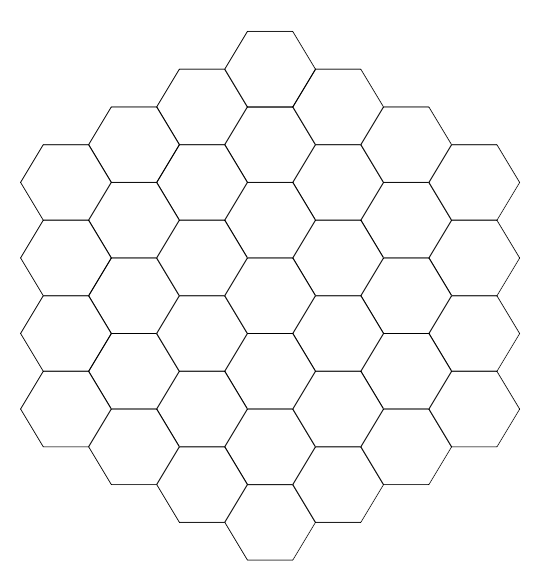
\includegraphics[width=0.45\textwidth]{cartedebase}
\end{figure}

\newpage

\subsection{Les créatures ou les pions du jeu}

La mythologie est un domaine où foisonne les créatures en tout genre. Idéal pour constituer un bestiaire. Surtout que les créatures diffèrent en fonction de la mythologie qu’on étudie, la mythologie égyptienne, grecque, celte. Les joueurs devront choisir une seule mythologie, possédant des caractéristiques uniques, parmi celles qui sont à leurs dispositions . Ils auront alors accès à un bestiaire propre à celle-ci. Ce fameux bestiaire sera une liste à laquelle le joueur pourra avoir accès tout au long du jeu. Il sera constitué de deux types de créatures: les basiques et les supérieures. Pour pouvoir créer

une créature supérieure les joueurs devront fusionner 3 créatures basiques nécessaire. Tant que les joueurs n’auront pas les éléments requis à la création de la créature supérieure celle-ci restera verrouillée dans le bestiaire en montrant ses besoins pour la déverrouiller. 

\subsection{L'invocation et les actions des créatures}

Le nombre de créatures sur la carte du jeu sera limité . Après la création d’une créature supérieure le joueur pourra invoquer des créatures de base pour combler son effectif. Cependant ses créatures seront créées dans une zone spéciale dans le camp du joueur que nous appellerons « spwan » pour qu’elles puissent rejoindre la partie il faudra que le joueur les déplace sur la carte principale du jeu. Chaque créature se voit attribuée une barre de mana. Ce mana sera utilisé par la créature dans ses déplacements et dans ses attaques. Cependant une créature ne pourra s’exécuter seulement de cette façon : se déplacer puis attaquer ou attaquer ou se déplacer uniquement. En fonction de la puissance de la créature elle aura des capacités spéciales et plus de points d’attaque. Les créatures se livreront des combats et celle qui aura le plus de points d’attaque gagnera et mangera la créature de l’adversaire.

\begin{figure}[!h]
	\center
	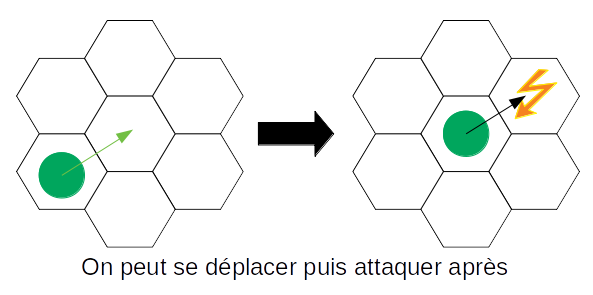
\includegraphics[width=0.6\textwidth]{deplaatta}
\end{figure}

\begin{figure}[!h]
	\center
	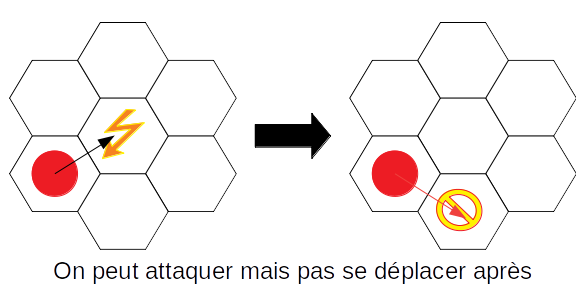
\includegraphics[width=0.6\textwidth]{attadepla}
\end{figure}

\subsection{Le déroulement du jeu}

La façon de jouer dans notre jeu sera très différente des autres jeux. En effet, ce ne sera pas un système en tour par tour ni un système en temps réel. Les joueurs devront jouer chacun leurs tours cependant la carte du jeu ne sera pas actualisée. Par exemple c’est au tour du joueur 1. Il va donner des actions à ses créatures et le joueur adverse ne pourra pas voir ses déplacements.Lorsqu’il aura fini, c’est le joueur 2 qui va à son tour choisir ses actions (invisibles par l’autre joueur). Les deux joueurs verront seulement la carte du jeu. Après avoir terminé leurs tours la carte s’actualisera et les joueurs pourront voir tous les mouvements qui ont été faits. Nous trouvons ce type de jeu plus intéressant car le joueur doit anticiper les mouvements de son adversaire. 

\section{Organisation}

\subsection{Répartition}

\begin{table}[!ht]
	\begin{center}
		\begin{tabular}{ | c || c | c | c | c | c | }
			\cline{2-6} \multicolumn{1}{c|}{}& Emmanuel & Marion & Léa & Antoine & Thibault \\ \hhline{-::=:=:=:=:=:}
			 Interface & x &&& \color{red} x & x \\ \hhline{-||-----|}
			 Personnages & x & x & \color{red} x & x & x \\ \hhline{-||-----|}
			 Graphisme && x & \color{red} x && \\ \hhline{-||-----|}
			 Son && x & x & x & \color{red} x \\ \hhline{-||-----|}
			 Plateau && \color{red} x && x & \\ \hhline{-||-----|}
			 Actions && x && \color{red} x & \\ \hhline{-||-----|}
			 Initialisation du jeu & \color{red} x &&&& x \\ \hhline{-||-----|}
			 Site internet & x && x && \color{red} x \\ \hhline{-||-----|}
			 Moteur & \color{red} x & \color{red} x &&& \\ \hhline{-||-----|}
			 LAN & x & x & x & x & \color{red} x \\ \hhline{-||-----|}
		\end{tabular}\\ 
	\end{center}
	\vspace{1cm}
	\textcolor{red}{x} : responsable\\
	x : suppléant
\end{table}

La première semaine de projet chaque membre du groupe va faire une recherche sur 6 créatures d’une même mythologie qu’il aura choisi auparavant. L’objectif étant de faire un récapitulatif de chaque créatures sous la forme d’une carte d’identité. On y affichera une photo (celle qui est la plus « juste » selon les sources), le nom, la mythologie, les caractéristiques et une petite description historique. 




l’interface du jeu : 
Gérer l’affichage des menus du jeu et l’emplacement des éléments graphiques. 

Déplacements et attaques :
Gérer les déplacements et les attaques des personnages.

Graphisme
Dessiner le portrait des personnages et l’aspect graphique du jeu.

Site internet
Créer le site internet qui servira à promouvoir notre jeu et donner les informations et ressources nécessaires.

Plateau
Créer plusieurs cartes de jeu prédéterminées et un mode aléatoire pour en diversifier l’expérience.

Son :
Ajouter les bruitages des personnages et la musique du jeu.

Initialisation
Initialiser les données de départ du jeu et récupérer des sauvegardes éventuelles.

Moteur
Collecter les données et les traiter pour passer au tour suivant.

\newpage

\subsection{Soutenances}

\begin{table}[!ht]
	\begin{center}
		\begin{tabular}{ | c | c | c | c | }
			\hline
			\multirow{12}{*}{Soutenance 1} & \multirow{2}{*}{Emmanuel} & Moteur & 20\% \\ \cline{3-4}
			&& Initialisation du jeu & 30\% \\ \cline{2-4}
			& \multirow{2}{*}{Marion} & Moteur & 20\% \\ \cline{3-4}
			&& Plateau & 25\% \\ \cline{2-4}
			& \multirow{2}{*}{Léa} & Personnages & 50\% \\ \cline{3-4}
			&& Graphisme & 25\% \\ \cline{2-4}
			& \multirow{2}{*}{Antoine} & Interface & 50\% \\ \cline{3-4}
			&& Actions & 20\% \\ \cline{2-4}
			& \multirow{2}{*}{Thibault} & Site internet & 30\% \\ \cline{3-4}
			&& LAN & 10\% \\ \cline{3-4}
			&& Son & 15\% \\ \hline \hline
			\multirow{12}{*}{Soutenance 2} & \multirow{2}{*}{Emmanuel} & Moteur & 60\% \\ \cline{3-4}
			&& Initialisation du jeu & 70\% \\ \cline{2-4}
			& \multirow{2}{*}{Marion} & Moteur & 60\% \\ \cline{3-4}
			&& Plateau & 75\% \\ \cline{2-4}
			& \multirow{2}{*}{Léa} & Personnages & 90\% \\ \cline{3-4}
			&& Graphisme & 65\% \\ \cline{2-4}
			& \multirow{2}{*}{Antoine} & Interface & 75\% \\ \cline{3-4}
			&& Actions & 60\% \\ \cline{2-4}
			& \multirow{2}{*}{Thibault} & Site internet & 60\% \\ \cline{3-4}
			&& LAN & 40\% \\ \cline{3-4}
			&& Son & 60\% \\ \hline \hline
			\multirow{12}{*}{Soutenance 3} & \multirow{2}{*}{Emmanuel} & Moteur & 100\% \\ \cline{3-4}
			&& Initialisation du jeu & 100\% \\ \cline{2-4}
			& \multirow{2}{*}{Marion} & Moteur & 100\% \\ \cline{3-4}
			&& Plateau & 100\% \\ \cline{2-4}
			& \multirow{2}{*}{Léa} & Personnages & 100\% \\ \cline{3-4}
			&& Graphisme & 100\% \\ \cline{2-4}
			& \multirow{2}{*}{Antoine} & Interface & 100\% \\ \cline{3-4}
			&& Actions & 100\% \\ \cline{2-4}
			& \multirow{2}{*}{Thibault} & Site internet & 100\% \\ \cline{3-4}
			&& LAN & 100\% \\ \cline{3-4}
			&& Son & 100\% \\ \hline
		\end{tabular}
	\end{center}
\end{table}

\section{Outils et moyens}

Pour ce projet nous allons utiliser les logiciels suivants :
\begin{itemize}[label=\textbullet]
	\item JetBrains Rider qui est un environnement de développement où l'on va faire le corps de notre jeu en C\#.
	\item VIM, Sublim text et Dreamweaver comme éditeur de texte lorsque l'on utilise un langage différent du C\#. Sublim text est une extension de VIM.
	\item Git et GitHub comme gestionnaire des différentes versions des fichiers faisant parties de notre projet. On pourra ainsi travailler en même temps sur le projet et facilement retouché une partie qu'on est seul a modifier à ce moment là.
	\item Audacity va être utiliser pour tout ce qui touche au son en créant ou modifiant des pistes audio pour la musique du jeu et les bruitages des personnages.
	\item Unity va permettre de traiter le graphisme du jeu simplement grâce à ses nombreux automatismes et raccourcis.
	\item Photoshop pour tout ce qui est traitement d'images déjà existantes.
\end{itemize}

En ce qui concerne le matériel nous allons travailler sur nos ordinateurs personnels, sur tablette graphique pour les graphismes des personnages ainsi qu'un micro pour enregistrer les bruitages des personnages.

\newpage

\section{Bonus}

Quand cela nous sera possible nous serons motivés pour créer le jeu en réseau afin que différentes personnes à travers le monde puissent s’affronter sur notre jeu. Mais étant donner la complexité de la tâche il est préférable que l’on laisse cela en tant que bonus pour nous focaliser sur l’essentiel du jeu.

\section{Conclusion}

Pour conclure ce cahier des charges nous espérons que notre concept en séduira plus d’un et que nous pourrions créer une petite communauté autour de celui-ci. Et si la magie noire nous maudit avec sa puissance nous allons la contrer avec notre magie blanche de la détermination. Pour préserver l’avenir de notre jeu et de notre équipe.

\end{document}
